\documentclass[runningheads]{llncs}

%---- Sonderzeichen-------%
%\usepackage {ngerman}
\usepackage[ngerman, english]{babel}
%---- Codierung----%
\usepackage[latin1]{inputenc}	% for Unix and Windows
\usepackage[T1]{fontenc}
\usepackage{graphicx}
\usepackage{url}
\usepackage{llncsdoc}
%----- Mathematischer Zeichenvorrat---%
\usepackage{amsmath}
\usepackage{amssymb}
\usepackage{enumerate}
% fuer die aktuelle Zeit
\usepackage{scrtime}
\usepackage{listings}
\usepackage{subfigure}
\usepackage{hyperref}

\setcounter{tocdepth}{3}
\setcounter{secnumdepth}{3}

\usepackage{lipsum}
\usepackage{graphicx}
\usepackage{tabularx}



\begin{document}
	
\newcolumntype{L}[1]{>{\raggedright\arraybackslash}p{#1}}

\mainmatter
%TODO Titel �ndern?????
\title{From Tradtitional Development to Continuous Deployment: Strategies and practices in CI/CD Pipelines}
\titlerunning{Deployment Strategies in CI/CD Pipelines}
\author{Niko Benkler }
\authorrunning{Model-driven Software Quality Engineering}
\institute{Supervisor: Dr. Robert Heinrich \\ \href{mailto:robert.heinrich@kit.edu}{robert.heinrich@kit.edu}}
\date{13.01.2018}
\maketitle

\begin{abstract} 
 	In the last decade, software development experienced a huge transition. Since agile methodologies were introduces in the early 2000, software development became faster and faster. Today, another software development process is emerging: Continuous Software Engineering (CSE). CSE, especially Continuous Integration(CI), Continuous Delivery(CDE) and Continuous Deployment(CD) receive more and more attention in organizations such as Facebook, Paddy Power and Atlassian but also in small start-up companies. 
 	It enables them to e.g. deliver software more frequently, reduce time-to-market, obtain customer feedback faster, build the right product or to improve product quality. 
 	Therefore, this seminar paper presents the current state of the art concerning Continuous Practices, compares the traditional deployment strategies with the new CSE practices and proposes some tools, that can be used in a CI/CD Pipeline to support CSE. But also, it reveals the barriers an organization has to face while adopting Continuous Practices. CSE not only turns up with benefits, it also has negative side effects such as a time consuming and costly implementation or an increasing mental stress for development team members.
 	% TODO: da fehlt noch was 10 scientific paper and a book were studied, in order to cover 
    \\
    
 	\textbf{Keywords - }Agile, continuous software development, continuous integration, continuous delivery, continuous deployment, DevOps, CI/CD Pipeline
 	 
	

\end{abstract}

\tableofcontents
\clearpage


\section{Introduction}
Today, the software development process has to face many difficult demands. Fast-changing and unpredictable markets, changing customer requirements \cite{claps2015journey} and rapidly advancing information technologies \cite{olsson2012climbing} require a faster process of software development. 
To achieve this, several organizations adopt Continuous Practices in order to extend their agile practices \cite{claps2015journey}. Therefore, releasing software becomes even faster. 
\\
This seminar paper presents a possible evolution path, referenced as 'stairway to heaven' \cite{olsson2012climbing}, which describes a transition from traditional development towards CD. 
As the core of CDE is a deployment pipeline \cite{schermann2016empirical}, the paper also presents its usual phases and the possible tools, that support each phase.
Nevertheless, studying several papers revealed, that CDE not only comes with benefits, but also with huge social and technical challenges \cite{claps2015journey}. The paper clarifies them and proposes some mitigation strategies. 
%TODO  Stimmt der remainder noch???
The remainder of the seminar paper is structured as follows: In section II, we define the terminology. Section III describes a possible transition from traditional deployment to CD based on the 'stairway to heaven' model \cite{olsson2012climbing} and \cite{shahin2017beyond}.This includes several deployment strategies used to adapt CSE practices and the comparison between traditional deployment and the CD process. That section is followed by an explanation of a possible pipeline and the available tools which can be used to support the tasks of each phase.  Section V discusses the challenges that are caused by CDE. Finally, I present my conclusion in section VI.

\section{Background} \label{background}
Here, I give an overview of the most important keywords. Those keywords are necessary to understand the content of the seminar paper. When studying the currently available information about Continuous Software Engineering (CSE), one could clearly see that there are no universally accepted definitions \cite{schermann2016empirical}. Terms like CDE and CD are sometimes used interchangeable, albeit the is a small but relevant difference \cite{shahin2017continuous}.
Therefore, the following subsections provide the definitions as they are used in this seminar paper.

\subsection{Agile Methodologies}
Agile software development is based on "iterative development, where requirements and solutions evolve through collaboration between self-organizing cross-functional teams" \cite{taheritanjani2016comparison}. It encourages adaptive planning, early delivery and continuous improvement.
Besides, other characteristics such as flexibility, efficiency, speed, the ability to react to fast changing customer requirements and fluctuating market needs \cite{olsson2012climbing} make agile methodologies so attractive for organizations. 
As mentioned before, agile methodologies were introduced in the early 2000 \cite{shahin2017continuous}. So far, many development companies succeeded in implementing agile methodologies. 
However, agile software development 'only' allows frequent software releases but no continuous releases. The difference becomes clear, when it comes to the comparison of traditional deployment and CD. 
The original "Manifesto for agile software development" popularized by Kent Beck did not include any automation. 

\subsection{DevOps}
 "\textbf{DevOps} is a set of practices intended to reduce the time between committing a change to a system and the change being placed into normal production, while ensuring high quality" \cite{bass2015devops}. It is a coined word, that stands for Development (Dev) and Operations (Ops). The main task is bringing together programmers, testers and quality insurance engineers but also  IT operations staff \cite{claps2015journey} to shorten feedback loop. According to \cite{bass2015devops}, the DevOps practices can be differentiated in 5 categories:
 \begin{itemize}
 	\item Treat Ops as "first-class citizens". This means, the involvement of operations in the development process. 
 	\item Dev has to be more responsible for incident handling to shorten the time between error observation an the error fix.
 	\item Include both, Dev and Ops into the deployment process in order to avoid errors caused by buggy deployment.
 	\item Use continuous deployment.
 	\item Use deployment scripts and other infrastructure code. This code is subjected to the same quality control practices than the application code. As a result, deployment error due to misconfiguration can be mitigated.
\end{itemize}

\noindent Especially the fourth category shows the close connection between DevOps practices and continuous practices.

\subsection{Continuous software engineering}
Continuous software engineering \textbf{(CES)} is a practice that promotes the development, deployment and the release of software products in very short cycles, typically hours or days. \cite{shahin2017continuous} \cite{taheritanjani2016comparison}. As a direct consequence, quick feedback allows i.a.: to determine new functionality to build, feature prioritization, information about the suitability of the current software architecture, to gather data for decision making in general. CES requires agile methodologies and DevOps practices \cite{taheritanjani2016comparison}. According to \cite{shahin2017continuous}, CES involves 3 phases: Business Strategy and Planning, Development, Operations. This seminar paper focuses on the three development activities: continuous integration, continuous delivery and continuous deployment. Fig. \ref{RelCSE} demonstrates the relationship between CI, CDE and CD.

\begin{figure}[h]
	\hspace*{-2cm} 
	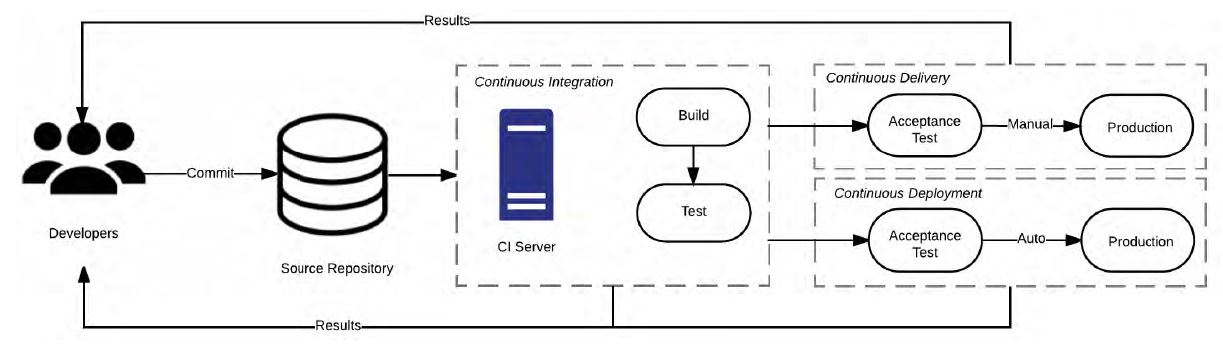
\includegraphics[height=4.5cm]{RelCSE}  
	\caption{\label{RelCSE}The relationship between CI, CDE, CD \cite{shahin2017continuous}} 
\end{figure}
\newpage

\subsubsection{Continuous Integration}
Continuous Integration \textbf{(CI)} is a CSE practice in which developers integrate and merge their work into a shared repository very frequently, for example multiple times a day \cite{shahin2017continuous} \cite{schermann2016empirical}. Also,  automated builds and tests permit to discover integration, build and test errors as fast as possible. CI improves  the effectiveness of a team as much as the software quality \cite{shahin2017continuous}. In other words, CI ensures, that the software is always in a ready to deploy state \cite{claps2015journey}.


\subsubsection{Continuous Delivery}
A brief definition of Continuous Delivery \textbf{(CDE)} is given in \cite{laukkanen2016bottom}: "Continuous Delivery is a software development discipline where you build software in such a way that the software can be released to production at any time." 
Preconditions for CDE are CI and a mechanism (e.g a tool) to automatically deploy and deliver software to a production like environment \cite{shahin2017continuous}. This practice has several benefits, such as a less risky release process \cite{laukkanen2016bottom} due to automation or the ability to learn from real usage data \cite{olsson2012climbing}. As a consequence, the software developers can decide whether it is worth continuing the work on a certain feature or discard it. As shown in Fig.\ref{RelCSE}, the release process is manually. This is concurrent with the definition of CDE, where it is mentioned that software 'can' be released automatically  instead of 'is' released. Therefore, CDE practice is classified as a pull-based approach, "for which business decides what and when to deploy" \cite{shahin2017continuous}.



\subsubsection{Continuous Deployment}
An extreme version of CDE is Continuous Deployment \textbf{(CD)}, where software 'is' actually released automatically. The goal of CD is to frequently deploy the software in a production environment. This happens for example several times a day (after each commit), one times a day (nightly build) or several times a week (weekend builds). Fig. \ref{CDBenefits}  provides a quick overview of CDE's and consequently CD's benefits. CD is a push-based approach \cite{shahin2017continuous}, as no manual task takes place in order to deploy the software to customer site. The CD (and CDE) practice is attained by using a deployment pipeline \cite{laukkanen2016bottom}, which is explained in Section IV. %TODO stimmt das mit der section? Auch n�chste Zeile
Whereas CD implies the usage of CDE practices, the inversion is not correct \cite{shahin2017continuous}.
Due to barriers such as "lack of automated (user) acceptance tests", "deployment as a business decision", "insufficient level of automated test coverage" \cite{shahin2017beyond} or the unsuitability of software types like embedded systems \cite{claps2015journey}, a forced transition from CDE to CD might not always be a good idea. This topic is discussed in Section 5 %TODO stimmt die section!

 \begin{figure}[h]
 	\centering
 	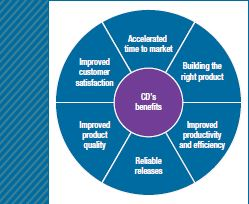
\includegraphics[height=4.5cm]{CDBenefits}  
 	\caption{\label{CDBenefits}CD's and CDE's Benefits \cite{chen2015continuous}} 
 \end{figure}




\section{The evolution path towards Continuous Deployment}
This section describes the transition from traditional development to Continuous Deployment and some main practices associated to these phases(Fig. \ref{Stairway}). Many software companies are subjected to constant alteration concerning their software development in order to stay competitive. Therefore, they need to improve their way of building software.
\\
 It is important to say that the application model plays a big role for the success of the CD adoption. Albeit the traditional 'waterfall model' may be still adequate for some companies offering legacy software (e.g in the financial sector), CD gains more and more attraction for Web-based applications \cite{schermann2016empirical}.
In the remainder of this section each phase of the "stairway to heaven" is discussed in detail. 
The barriers each transition causes, are discussed in section V. %TODO stimmt das? 

\subsection{The Stairway to Heaven}
The main ideas within this section come from \cite{shahin2017continuous}, \cite{schermann2016empirical} and \cite{olsson2012climbing}. They refer to CD as a practice to keep the product "perpetually in a shippable state" using a "fully or at least partially automated deployment pipeline" \cite{schermann2016empirical}. This shows the interchangeability of CDE and CD as they are combining CDE and CD in one term. Besides, they put another practice on top of CD: "Partial Rollouts" (Fig.\ref{Stairway}). 
 \cite{schermann2016empirical} also points out that the adoption of CD does not always has to follow the "stairway to heaven" as many companies already implemented a few continuous practices.

\begin{figure}[h]
	\hspace*{-2cm} 
	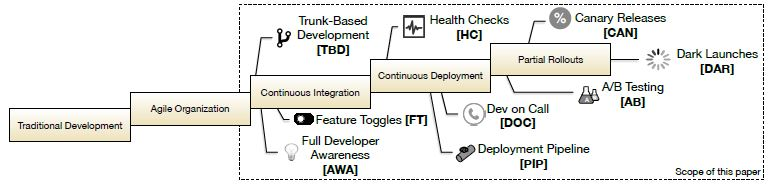
\includegraphics[height=4cm]{Stairway}  
	\caption{\label{Stairway}The "stairway to heaven", and the main practices associated to the phase in this evolution step\cite{schermann2016empirical}} 
\end{figure}


\subsubsection{Phase 1: Traditional Development}
Traditional deployment is a software development approach, that is characterized by slow development cycles, the "waterfall model"  or a bad customer integration \cite{olsson2012climbing}.  The delivery and deployment process is typically at the end of the project. Usually, the developed software is formed as a monolithic 3-Layer architecture with all the included disadvantages. It has to be noticed, that it is not the aim of the seminar paper to judge about the suitability of this kind of software development and architecture. But for successfully implementing Continuous Practices, they are simply not suitable \cite{claps2015journey} \cite{shahin2017continuous} \cite{shahin2016intersection} \cite{shahin2017beyond}. The next step in software evolution in agile organization. 

\subsubsection{Phase 2: Agile Organization}
A brief introduction in Agile Methodologies is given in \ref{background}. Agile Organization, of course, includes agile methodologies, but "product management and system verification still work according to the traditional development model" \cite{olsson2012climbing}.
To successfully proceed to agile organization, the most important aspect is mindset. The resistance to change is a challenge for each evolution step. Therefore, managerial support is needed to convince each employee of the initiative. Having a few agile teams promoting their methods within the organization, has a positive effect on the whole company \cite{olsson2012climbing}. Besides, there is a strong need to improve information exchange within and across the teams. As a result, the development teams are organized in small and cross-functional teams. The members of cross-functional teams covers all aspects of software development and delivery \cite{taheritanjani2016comparison}. This enables the organization having feature teams instead of component teams. Feature teams work on complete features which supports iterative development. As a consequence, this improves the release frequency. It has to be noted, that the development teams do not yet continuously integrate their code to a organization-wide shared code base. So far, they develop a feature within their team and when it passes all required test, they merge it into the main project. 
\\ 
The next step of the "stairway to heaven" is Continuous Integration. The following subsection provides some basic concepts to achieve CI. 

\subsubsection{Phase 3: Continuous Integration}  
The core of CI is the continuous integration of code into a shared repository across all teams developing a software product. Again, a cultural shift is necessary in order to realize CI practices \cite{olsson2012climbing}. Branching strategies like trunk-based development (TBD), the implementation of feature toggle (FT) or the concept of full developer awareness (AWA) facilitate practising CI. The continuous integration of code by many different teams can result in long-living parallel development branches . To reduce this complexity, \cite{schermann2016empirical} proposes trunk-based development, where all teams integrate into one single branch, called master branch or master trunk. What happens to features that are not ready to be deployed, but already integrated into master? The concept of Feature Toggles provides a good solution strategy. In very simple terms, Feature Toggles permit to switch on or off a certain code block. So whenever a feature is ready for production, you just turn it on. Another concept to enable and promote full transparency of the project (e.g build status, test coverage, latest client version or status and progress of features) is called (full) Developer Awareness(AWA). AWA is realized by Dashboards, public monitors in the office or chat tools informing everybody and creating transparency.
\\
Fig. \ref{RelCSE} demonstrates, that not only code integration, but also automated builds and test play a huge role in Continuous Practises, especially CI. Adopting "test-driven development" (TDD), "test planning" and "cross-team testing" improves the test phase during CI. TDD is a process in which requirements or user stories are turned into very specific tests. It is divided into 4 different steps: 1. Add a test based on a required feature, 2. Run all test and see which test fails, 3. Write or refactor the code, 4. Run the tests again. Repeat those steps in very short development cycles until all test cases are passing. This helps to continuously check the quality of the written code. "Test planning" is a concept to intensify the collaboration between Quality Assurance (QA) and developers according to the DevOps principles. Together, they make a comprehensive list of automated tests. This "liberates QAs from manually testing the majority of the software application for regression bugs" \cite{shahin2017continuous}. In "cross-team testing", tests are performed by a group of developers from another team and vice versa. 
\\
Besides, defining new roles like a build sheriff is a useful practice to promote  CI's success.
The build sheriff constantly watches the CI process or indicates that build process failed \cite{shahin2017continuous}.

\subsubsection{Phase 4: Continuous Delivery and Deployment}
As mentioned in the introduction of this section, CD is a practice to keep the product "perpetually in a shippable state" using a "fully (CD) or at least partially(CDE) automated deployment pipeline" \cite{schermann2016empirical}. The core practice of CD, the deployment pipeline, is discussed  in section IV. %TODO: Stimmt das?
CD requires not just the development and operations team (DevOps), but also the product management as an interface to the customer. \cite{olsson2012climbing}. \cite{shahin2017continuous} claims that work structures have to be clarified. There is a need of defining new roles and teams when adopting CD, such as a release coordinator or release manager. Fig. \ref{teamstructure} demonstrates a potential team structure as it can be found in an software developing organization using CSE for their multiple projects.

\begin{figure}[h]
	\centering
	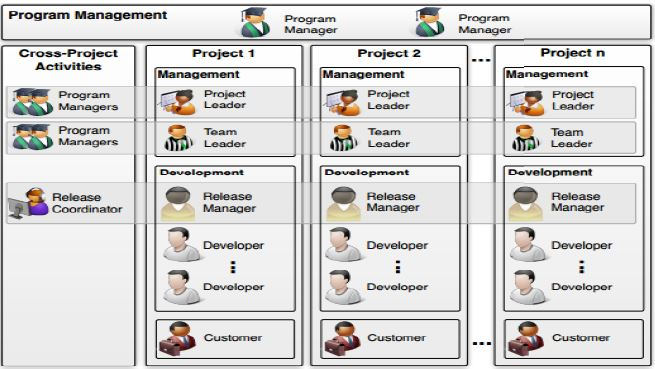
\includegraphics[height=4cm]{teamstructure}  
	\caption{\label{teamstructure}Possible team structure in a CSE Team  \cite{taheritanjani2016comparison}} 
\end{figure}

Further practices to successfully implement CD are "health checks" (HC) and the idea of "developer on call"(DOC). Monitoring on infrastructure (e.g CPU utilization) and application (e.g response time) level is used to extinguish 'health' problems of the deployed software. Those "health checks" can also be used to support rollout decisions (e.g increase traffic for a canary release) \cite{schermann2016empirical}. "Developer on call" is associated with the idea of DevOps: Developers shall be available and responsible for their code, all the more after deployment. In case of any error occured after a code change, they know best where to find and how to fix it.

\subsubsection{Phase 5: Partial Rollouts}
\cite{schermann2016empirical} describes partial rollout practices as "the epitome" of CD. Releasing software is always the critical part in software engineering, as customers may receive buggy code. So what can be done to mitigate the consequences of deploying buggy software? \cite{shahin2017continuous} and \cite{schermann2016empirical} propose the usage of "canary release", "A/B Testin"(AB) or "Dark Launches"(DAR). Those practices are considered as "run-time quality assurance and requirements validation techniques" \cite{schermann2016empirical}.
\\
Canary Release is a deployment method where a new software version is deployed only to a "small set of users". That mitigates the influence of possible buggy code and at the same time produces some real usage data. With that, a team decide if either the released version needs further improvement or can be released completely. A variation of canary release is the "eat your own dog food" approach, where only internal organization members get to use the new version.
%TODO: Umsetzungsarten k�nnen hinzugef�gt werden
\\
A/B Testing is similar to canary release. It requires a bigger user base, as there are currently two versions running. By collecting statistics, the team is able to decide whether version A or B performs better.
\\
Dark Launching is the process of deploying functionality to production in order to test it, but with limited or no access for any users. This enables the team to test new functionality in the production environment and consequently decide, whether the feature is ready to "handle production-scale traffic" \cite{schermann2016empirical}. To dark launch a feature, the team implements the old and the new feature with Feature Toggles and decides which one to show to the user. 

\subsection{A comparison between traditional development, agile development and the CD process}
The following table compares the development and deployment of the traditional, agile and CD process based on \cite{claps2015journey}.

\begin{table}
	
\begin{tabular}{|L{2.5cm}|L{3cm}|L{3cm}|L{3.5cm}|}

\hline
  & Traditional development & Agile development & Continuous Practices \\
 \hline
 Team size & Big Teams, a few dozen poeple & Small teams, 2-8 people & Small teams, 2-8 people \\
  \hline
 Team competence & Divided in discipline  & Cross-functional teams & Cross-functional teams and new roles\\
  \hline
 Planning & Rigorous planning phase at the beginning & Iterative planning in short cycles & Continuous planning in short cycles\\
  \hline
 Testing & Explicit testing at the end of the project   & Testing at the end of each cycle & (Semi-)automated tests with every pipeline run  \\
  \hline
 Architecture & 3-Layer, monolithic, strong dependencies between modules & 3-Layer or Microservices, less dependencies & Desire: almost no dependencies, independent deployability of modules    \\
  \hline
 Frequency of deployment & Once waterfall process finished (months, year) & Weekly & Daily  \\
  \hline
 Relative risk of deployment & High: no automation, infrequent process, huge amount of code & Still High: no automation but frequent process  &Low: automation, small amount of changes, only few dependencies \\
  \hline
 Customer/developer feedback loop & Long due to infrequent deployments & Depends on the deployment frequency &Very short, customers constantly give feedback\\
  \hline
 Unnecessary features & High amount due to long feedback loop & & prevent development of any wasted software  \\
 \hline
\end{tabular}
\end{table}

\section{Deployment Pipeline and Tools}
A Deployment Pipeline is considered to be the core of the CSE process. It enables organizations to automate code integration, build process, testing, configuration and deployment. Common stages of CD/CDE pipelines are "version control", "build", "continuous integration","artifact repository management", "unit/integration/acceptance/performance testing", "deployment", "configuration and provisioning", "log management and monitoring", "containerization" or "issue tracking" \cite{shahin2017beyond} \cite{taheritanjani2016comparison}. The vast amount of possible stages demonstrate, that there is no universally applicable pipeline. \cite{chen2015continuous} goes even further: Pipelines should be redesigned for each application to best suit the needs.
\\
Nevertheless, the main idea of a pipeline in CDE is always the same: Moving from stage to stage is (at least semi-)automated. If any error occurs, the pipeline stops and notifies the development team. They are able to fix it and start the pipeline again by committing the changes. 
\\
Thus, the engineering process of a pipeline,the software's architecture, the degree of automation or the available tools generate some serious challenges. They are discussed in Section V.

\subsection{Example: A deployment pipeline} 
The example pipeline is divided in 7 stages: 1. version control system, 2. code management and analysis, 3. build system, 4. continuous integration server, 5. testing, 6. configuration and provisioning, 7. continuous delivery/deployment server \cite{shahin2017continuous}.

\begin{figure}[h]
	\centering
	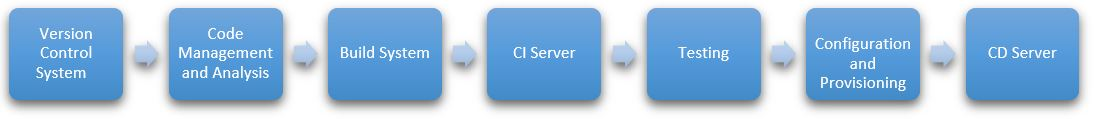
\includegraphics[height=1.2cm]{pipeline}  
	\caption{\label{pipeline}Deployment Pipeline based on \cite{shahin2017continuous} } 
\end{figure}

\subsubsection{Version Control System}
The Version Control System manages the continuous code pushing to the repository. It tracks files to create a history of the development process. The most popular ones are GitHub and Subversion. GitHub Issues as Issue Tracking software can be integrated here as well. \cite{taheritanjani2016comparison}.
\subsubsection{Code Management and Analysis}
Code Management and Analysis tools check the code concerning static quality metrics. Those can be: code and test coverage, coding standards like comments, alignment or duplicated code. SonarQube is on of the most popular tools, as it can be fully integrated in CI environment \cite{shahin2017continuous}.
\subsubsection{Build System}
Build tools simplify the build process. They compile the source code automatically into binary code and packages. Popular Tools are Apache Maven or Ant.
\subsubsection{CI Server}
The CI server observes the code repository. According to the respective build policy, it triggers the Build System and runs the tests whenever a change is committed. Bamboo, Jenkins and Travis CI are the most common CI Server tools.
\subsubsection{Testing}
Testing is the key aspect to guarantee high qualitative software. This leads in various different kinds of tests: Unit tests, regression tests, (user) acceptance tests, integration test or performance tests.
\\
JUnit is a common tool to run unit tests. To store the results of acceptance tests, \cite{shahin2017continuous} proposes the test management framework TestLink. Besides, the CRTS(Continuous Regression Test Selection) and CTSP(Continuous Test Suite Prioritization) approaches intend to support effective regression test within the CI server environment. The combination  of CUTS and CruiseControl (CI Server tool) is used to continuously run system integration tests.


%TODO: wohin damit?Albeit developers already succeeded in automating unit and integration tests, the automation of (user) acceptance tests and performance tests remains a big challenge.



\subsubsection{Configuration and Provisioning}
Automating the configuration and provision of servers, test environments, virtual machines or infrastructure is an innovation in deployment pipelines \cite{shahin2017continuous}. Usually, a vast amount of time is needed to set up those environments \cite{chen2015towards}. This justifies that new approach, albeit there a currently not that many tools available. 

\subsubsection{CD Server}
The release process of a software is the final stage in Continuous Software Engineering(CSE). Having a tool that automatically deploys code to production (either internally or externally) is substantial for successfully accomplish the goal of CSE.
\\
HockeyApp is a well known CDE server. Web Deploy or Deployr are software tools to automatically deploy code to production. \cite{shahin2017continuous}.



\subsection{Tools in a Deployment Pipeline}
Fig.\ref{Tools} provides some tools and divides them into the stages they belong to. Some of them are expensive enterprise tools, others are Open Source. This seminar paper does not aim to give a detailed explanation or comparison of those tools, as this would be far to complex. 

\begin{figure}[t]
	\centering
	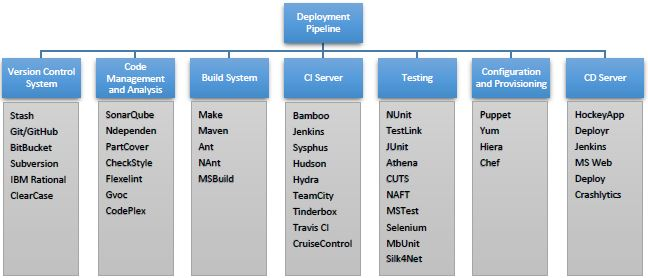
\includegraphics[height=5.5cm]{Tools}  
	\caption{\label{Tools}An overview of tools used to form a deployment pipeline \cite{shahin2017continuous} } 
\end{figure}

\newpage

\section{Challenges for Adopting Continuous Practices}
"Continuous Delivery: Huge Benefits, but Challenges Too" \cite{chen2015continuous}. This is how Lianping Chen, a software developer of a company called Paddy Power, names his paper. He describes how they (Paddy Power) adopted Continuous Practices, reporting "huge benefits and challenges involved".
\\
While studying several papers about Continuous Practices in general, it was remarkable how many of them reported about the challenges of adopting CI,CDE or CD. 
Currently, there is little research done on how to better introduce them \cite{chen2015continuous}.  As a consequence, "out of the box" solutions are mostly not available.
\\
The following sections are divided in the different kinds of challenges a software development organization may has to face when adopting Continuous Practices
Those are: Organizational, technical, social and architectural challenges. If available, mitigation strategies are provided as well.


\subsection{Organizational Challenges}
Almost every source identifies the breakdown of barriers among the teams as on of the most important organizational challenge. For successfully adopting Continuous Practices, transparency, coordination and a closer collaboration between development teams, operational staff and management has to be established. Team restructuring and the definition of new roles are common mitigation practices \cite{chen2015continuous}. To establish more transparency, full developer awareness is required, as mentioned in Section II.
\\
Having separated development and operation staff causes a very slow failure recovery \cite{shahin2016intersection}. The introduction of DevOps practices reduces the time between failure discovery and bug fix according to the principle: "You build it, you run it" \cite{shahin2016intersection}. 
Deployment is a business decision. In Some organizations, only management or financial operators are in charge of the release decision. Asking for permission to release can be a lengthy process, which is obviously contrary to the idea of CD \cite{shahin2017beyond}.
The same source identifies the lack of experience and skill as another challenge. Using pilot teams, formal training and workshops is a counteracting strategy.



\subsection{Technical Challenges}
The variety of available tools to implement Continuous Practices is problematic. Especially test tools for user acceptance test are either non-existent or hardly capable of being integrated into an automated pipeline \cite{shahin2017beyond}. Besides, manual quality checks are sometimes unavoidable. A fully automated testing infrastructure still is one of the main challenge to achieve full automation \cite{laukkanen2016bottom}.
\\
As there are no "out of the box" solutions, companies have to design and implement their own CD pipeline. A "no downtime policy" requires proper hardware, as seamless upgrades are necessary. It is simply not possible, to shut down the system, every time a new version is deployed. This is not just time consuming but connected to a high investment which discourages companies to do CSE \cite{chen2015continuous}.  \cite{shahin2017continuous} reports that security issues in pipeline still remain a big challenge. 
It has to be noted, that some domains do not allow to truly implement CD. E.g. embedded systems, telecommunication systems, medical and other safety critical systems.





\subsection{Social Challenges}
The resistance to change or the lack of motivation are obstacles while adopting Continuous Practices \cite{chen2015continuous} \cite{claps2015journey}. To address these barriers, it has to be ensured that team leaders and managers are pushing the new practices and convince their employees of the benefits. Pilot teams and workshops may help to better introduce CSE within the company.
Nevertheless, it has been reported that the pressure on developers increases, as the are in charge of having the code always ready for production. 
Mistrust in the build process and the test results are a common reason for developers to reject CSE \cite{laukkanen2016bottom}. Therefore, confidence into the CD process has to be established. 
\\
At customer site, demotivated  clients make it difficult to introduce Continuous Practices. They need to be involved in the release process, which they primarily consider as a time consuming task \cite{shahin2017beyond}. 





\subsection{Architectural Challenges }
\cite{chen2015continuous}
- large, monolithic apps => redesign, but costly \cite{schermann2016empirical}


\cite{shahin2016intersection}
- highly coupled monolitic architecure hav cross functional dependencies which need to be managed in pipeline => vey diffivult
- monolith database undeployable unit =>aplitting into smaller and less complex databases
=> small independent deployment units MIccroservice, vetical layering
=> do not focus on reusability as this creates dependencies / bottleneck
=> testability inside the architecture. Test services stand-alone




\newpage

\bibliographystyle{itmalpha}
% TODO: �ndern der folgenden Zeile, damit die .bib-Datei gefunden wird
\bibliography{literatur}

\end{document}

